\documentclass{article}
\usepackage{tikz}

\begin{document}

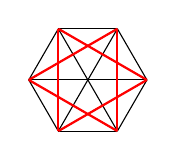
\begin{tikzpicture}[scale=1.5]
    % Define the vertices of the dodecahedron
    \foreach \i in {0,...,5} {
        \pgfmathsetmacro{\theta}{60*\i}
        \pgfmathsetmacro{\phi}{2*atan(1/sqrt(3))}
        \coordinate (A\i) at ({cos(\theta)*cos(\phi)}, {sin(\theta)*cos(\phi)}, {sin(\phi)});
    }
    
    % Draw the edges of the dodecahedron
    \foreach \i in {0,...,5} {
        \foreach \j in {\i,...,5} {
            \draw[black] (A\i) -- (A\j);
        }
    }
    
    % Draw the red edges connecting opposite vertices
    \foreach \i in {0,...,5} {
        \pgfmathtruncatemacro{\nexti}{mod(\i+2, 6)}
        \draw[red, thick] (A\i) -- (A\nexti);
    }
\end{tikzpicture}

\end{document}